\chapter{Kalimantacin ACP swap in mupirocin cluster}
\label{cha:chap4}

\section{Introduction}
\label{sec:chap4-Intro}
The predicted structure of the ACP-MupH complex, described in the previous chapter, highlighted various key residues important for the ACP-HCS recognition required for \bet-branching. Tyrosine 62 on helix III in ACP-mupA3ab was predicted to be at the interface of the interacting models. Mutating Y62 to F or A in the $ \Delta $ACP-mupA3b strain reduced mupirocin production by four and ten fold respectively, as determined by HPLC. This loss in function confirmed the importance of helix III of the \bet-branching ACPs for the formation of a functional complex with an HCS protein. However, later experiments showed reduced complementation by \textit{batC} (kalimantacin cluster) in a $ \Delta $\textit{mupH} strain. Interface residues identified in the ACP-MupH complex included residue 219 on MupH which was a methionine in MupH and TmlH (thiomarinol cluster) but a leucine in BatC. BatC L218M has an improved ability to complement $ \Delta $\textit{mupH}, with three fold more mupirocin production compared to wild type BatC. This observation suggested that although the \bet-branching ACPs usually have a conserved tryptophan in the core, and a Y on helix III forming the interaction interface, there exists ACP-HCS pairwise subtype specificities. This pairwise specificity can be observed in the myxovirescin system where there are two sets of HCS cassettes that interact with their cognate ACPs.

Extending the observation that \textit{batC} failed to complement $ \Delta $\textit{mupH} in the mupirocin cluster due to a difference in the interaction specificity, it seemed that swapping ACP-mupA3ab in the mupirocin cluster with the \bet-branching ACP(s) from the kalimantacin cluster should also fail. However, it should be possible for complementation of ACP-mupA3ab by kalimantacin ACP(s) upon changing the residues at its interface, or if the kalimantacin ACPs were expressed together with the wild type \textit{batC} in the mupirocin system. Thus here, the kalimantacin ACP (ACP-K24a; K=kalimantacin, 2=second protein, 4=fourth module, a=first ACP) was amplified from a purified DNA sample obtained from our collaborators. The idea behind selecting ACP-K24a was that it was one of tandem ACPs similar to the branching ACPs in the  mupirocin cluster and it seemed to be performing only the addition of a methyl branch without any other modifications that were present in the other \bet-branching sites in the kalimantacin cluster. Two host strains,  \textit{P. fluorescens} $ \Delta $\textit{acp4} and \textit{P. fluorescens} $ \Delta $\textit{mupH} were used. The \textit{P. fluorescens} $ \Delta $\textit{mupH} strain lacks \textit{mupH} in the HCS cassette and was used to express \textit{mupH}, \textit{batC} and \textit{batC} L218M \textit{in trans}, described in detail in section \ref{sec:bactstrains}. 

\section{Results}
\label{sec:chap4-results}
	
	\subsection{Plasmid preparation and transfer for Suicide Mutagenesis}
	
	\subsubsection{Amplification of DNA fragments for ligation into a pAKE 604 suicide plasmid}
	\label{sec:chap4PCRresults}
	Replacement of the branching ACPs in the mupirocin pathway with kalimantacin ACP-K24a was through homologous recombination via suicide mutagenesis. A pAKE604 plasmid was used to clone DNA fragments from the mupirocin and the kalimantacin cluster. To ensure that sequence amplified for ACP-K24a includes all the secondary structures for an ACP, a sequence length equivalent to the length of the solved ACP-mupA3a structure was taken for PCR primer construction. For homologous recombination to happen ACP-K24a needs to be attached to the $ \approx$500 nucleotide long arms either side of the mupirocin cluster ACP-mupA3ab. The left and the right arms were amplified from both the ends of the ACP-mupA3a sequence using the \textit{P. fluorescens} $ \Delta $\textit{acp4} strain as the template. The details of the PCR setup and the primers used are described in section \ref{sec:pcr}. 
	
	The amplified fragments were analysed using 1\% agarose gel electrophoresis and were purified using the GE Healthcare Life Sciences Illustra-GRX PCR DNA and gel band purification kit. Figure \ref{fig:threefragments} shows the purified fragments for the left arm, right arm and ACP-K24a on the agarose gel. The concentration of the purified samples were quantified using the Nanodrop instrument in order to calculate the volume of samples to be used in the Gibson assembly reaction described later. Simultaneously, a pAKE604 vector was cut using two restriction enzymes (HindIII and SalI) at the multiple cloning site and the concentration of the purified product was also quantified using the Nanodrop instrument.  
	
		\setlength\fboxsep{5pt}
		\setlength\fboxrule{1.5pt}
		\begin{figure}[htbp]
		\centering
		\fbox{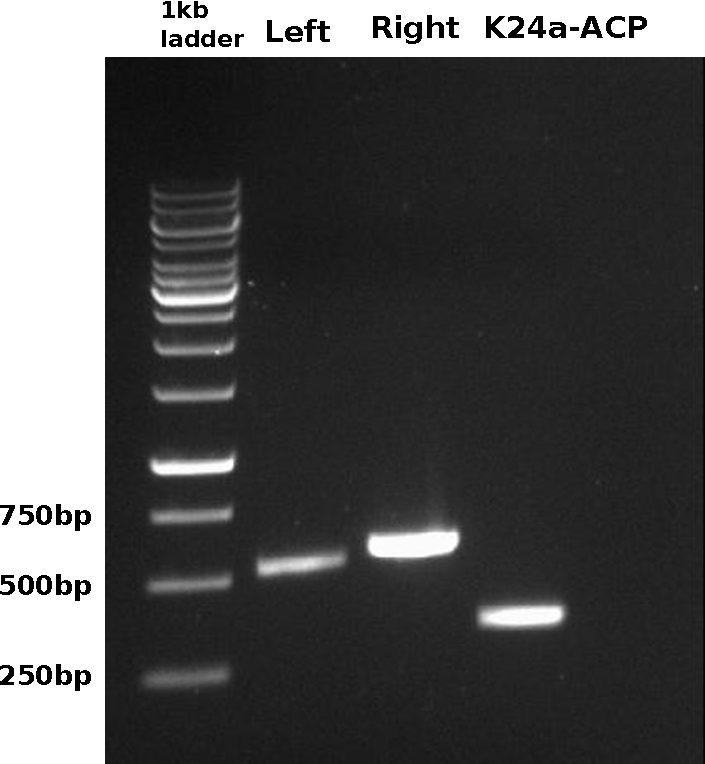
\includegraphics[keepaspectratio=true]{graphics/threefragments.pdf}}
		\caption[Purified fragments for the left arm, right arm and ACP-K24a on agarose gel.]{Purified fragments for the left arm, right arm and ACP-K24a on agarose gel. The size of the fragments include the homology regions required for Gibson assembly.}
		\label{fig:threefragments}
		\end{figure}
	
	\subsubsection{DNA fragments ligation into pAKE604 using Gibson assembly}
	\label{sec:chap4gibson}
	Gibson assembly is a method to ligate several DNA fragments in a single reaction (details in section \ref{sec:gibson}). In order to perform the ligation of the ACP-K24a to the two ACP-mupA3ab flanking arms and the multiple cloning site of pAKE604, a Gibson assembly kit from NEB was used. %For Gibson assembly NEB recommends a total DNA concentration of 0.2 to 1.0 pM when 4 to 6 DNA fragments are to be assembled. 
	The DNA concentration calculated for ACP-K24a was 68.1 ng/$ \mu $l, for the left arm it was 50.8 ng/$ \mu $l, for the right arm it was 98.1 ng/$ \mu $l and for the digested pKAE604 it was 121 ng/$ \mu $l. For the ACP-K24a of length 297 the volume required was 0.8 $ \mu $l, for the left arm of length 487 was 1.5 $ \mu $l, for the right arm of length 532 was 0.9 $ \mu $l and for pKAE604 of length 7219 was 9.7 $ \mu $l. Since the total amount of solution required for one Gibson assembly reaction was 20 $ \mu $l which include 10  $\mu $l of the Gibson assembly master mix the total volume of the three DNA fragments excluding vector was scaled down to 3 $ \mu $l from 3.2 $ \mu $l and the volume for the vector was scaled down to 7 $ \mu $l from 9.7 $ \mu $l. Volume equal to two Gibson assembly reactions was measured and split into three tubes of 13 $ \mu $l, 14 $ \mu $l, 13 $ \mu $l each and were incubated at 45\textcelsius,  50\textcelsius \ and 55\textcelsius \ respectively for one hour. The standard NEB manual protocol did not yield any ligated product so an alternative method for Gibson assembly was tried. The reaction mix prepared for the total volume of two reactions was divided into three tubes, which were incubated at three different temperatures. The three temperatures were 45\textcelsius,  50\textcelsius \ (recommend by NEB) and 55\textcelsius. The contents of the three reaction tubes were then pooled into a single tube  and the mix was then used for transforming the freshly prepare \textit{E. coli} DH5$ \alpha $ competent cells (section \ref{sec:compcell} and \ref{sec:transformation}) as recommended in the NEB Gibson assembly protocol. The idea behind pooling all the content into one tube was to reduce the transformations to be done for each temperature, if the Gibson assembly worked for any of the temperatures then the assembled plasmid should be taken up by the competent cells and only the transformed cells would survive the kanamycin selection. A disadvantage of this method is that which temperature(s) actually worked amongst the three remains unknown.
	
	The transformation plates showed fourteen colonies in total which were streaked to single colonies. From the streaked plates fourteen colonies were picked, one for each of the original fourteen streaks, and the PCR was performed using the left arm forward primer and the right arm reverse primer. Out of the fourteen samples, eleven gave DNA fragments of the required size as analysed on 1 \% agarose gel electrophoresis (Figure \ref{fig:gibsongel}). Four of the eleven successful PCR products were purified and two of these were sequenced using primers designed previously by Dr. Joanne Hothersall, which bind to the region outside the multiple cloning site of the pAKE604 plasmid. Of the two samples the forward and reverse reads for the second sample showed the expected sequence. The validated second sample was used to transform freshly prepared \textit{E. coli} S17-1 competent cells.

		\setlength\fboxsep{5pt}
		\setlength\fboxrule{1.5pt}
		\begin{figure}[htbp]
		\centering
		\fbox{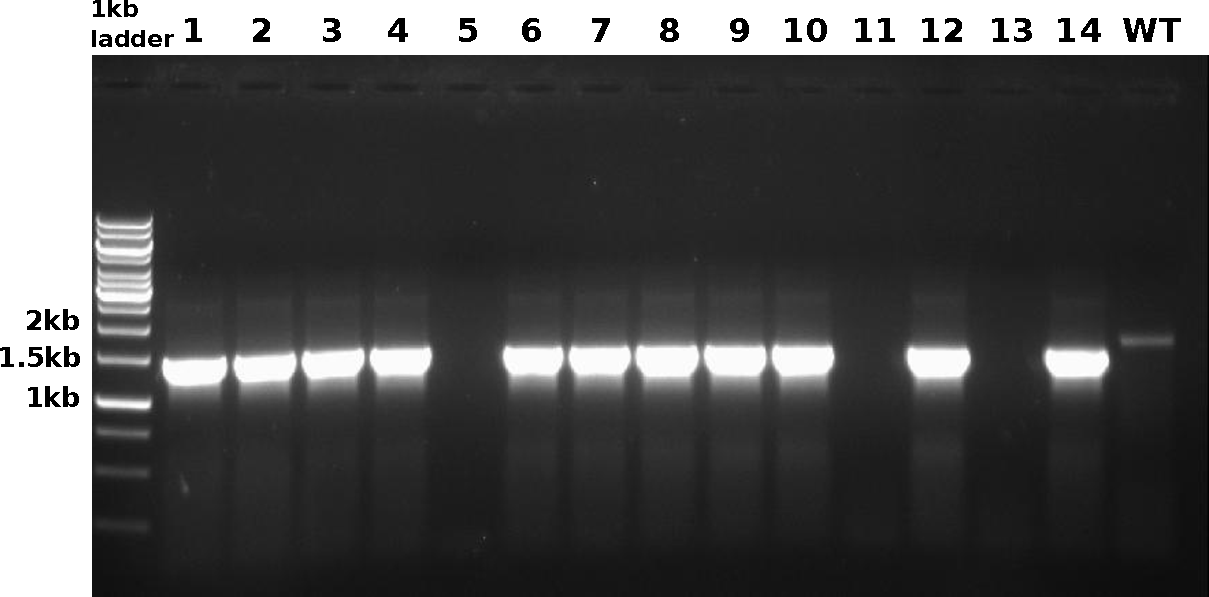
\includegraphics[width=0.9\textwidth,keepaspectratio=true]{graphics/gibsongel.pdf}}
		\caption[Gibson assembly product on agarose gel.]{Gibson assembly product on agarose gel. Eleven out of fourteen samples showed the right size band of roughly 1.5 Kb in size. \textit{P. fluorescens} NCIMB 10586 was used as control and the amplified product contains both ACP-mupA3a/b.}
		\label{fig:gibsongel}
		\end{figure}

	\subsubsection{Conjugal transfer of the suicide plasmids into \textit{P. fluorescens} host strains}
	\label{sec:chap4mating}
	The suicide plasmid pAKE604 carrying the construct \textquotedblleft left arm - ACP-K24a - right arm\textquotedblright \ in \textit{E. coli} S17-1 was transferred to two different \textit{P. fluorescens} strains through mating. The strains were \textit{P. fluorescens} $ \Delta $\textit{acp4} and \textit{P. fluorescens} $ \Delta $\textit{mupH} (details in section \ref{sec:mating}). Trans conjugants were subjected to PCR using the ACP-K24a specific primers to detect the successful transfer of the plasmid into \textit{P. fluorescens} $ \Delta $\textit{acp4} and $\Delta $\textit{mupH} cells.
		
	For \textit{P. fluorescens} $ \Delta $\textit{acp4} trans conjugants eight colonies were subject to PCR along with non mated \textit{P. fluorescens} $ \Delta $\textit{acp4} and transformed \textit{E. coli} S17-1 strains as negative and positive controls respectively (Figure \ref{fig:delta4conju}). All the colonies as well as the positive control showed the presence of the plasmid sequence. 
	
		\setlength\fboxsep{5pt}
		\setlength\fboxrule{1.5pt}
		\begin{figure}[htbp]
		\centering
		\fbox{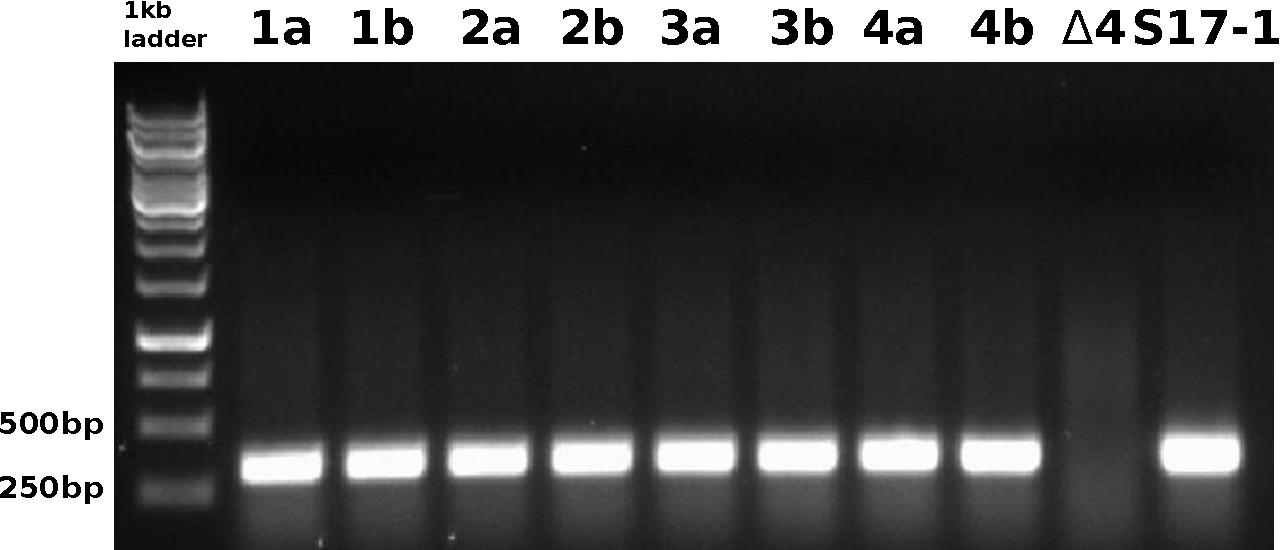
\includegraphics[width=0.9\textwidth,keepaspectratio=true]{graphics/delta4conju.pdf}}
		\caption[Validation of \textit{P. fluorescens} $ \Delta $\textit{acp4} trans-conjugants.]{Validation of \textit{P. fluorescens} $ \Delta $\textit{acp4} trans-conjugants. All the eight colonies as well as the positive control showed the presence of the plasmid carrying the ACP-K24a. No band was detected for the negative control.}
		\label{fig:delta4conju}
		\end{figure}		
		
	For \textit{P. fluorescens} $ \Delta $\textit{mupH} trans-conjugants ten colonies were subjected to PCR along with a transformed \textit{E. coli} S17-1 strain as a positive control (Figure \ref{fig:deltahconju}). Nine out of ten colonies as well as the positive control showed the presence of the plasmid sequence.

		\setlength\fboxsep{5pt}
		\setlength\fboxrule{1.5pt}
		\begin{figure}[htbp]
		\centering
		\fbox{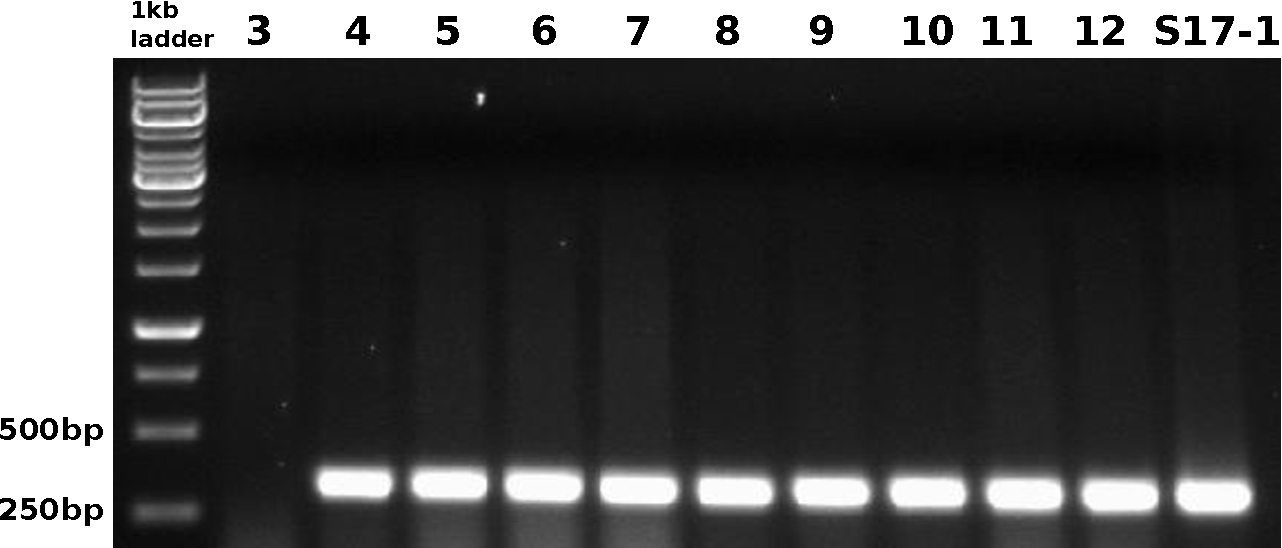
\includegraphics[width=0.9\textwidth,keepaspectratio=true]{graphics/deltahconju.pdf}}
		\caption[Validation of \textit{P. fluorescens} $ \Delta $MupH trans-conjugants.]{Validation of \textit{P. fluorescens} $ \Delta $MupH trans-conjugants. Nine out of ten colonies as well as the positive control showed the presence of the plasmid.}
		\label{fig:deltahconju}
		\end{figure}

	\subsection{Sucrose selection and excisant validation}
	\label{sec:chap4suc selection}
	%After mating, the \textit{P. fluorescens} trans-conjugants should have allowed the plasmid to integrate into the mupirocin cluster. by growing them overnight in L-broth without any selection (see details in section \ref{sec:suc selection}). The $ \approx $500 bp arms attached to the ACP-K24a would guide the homologous recombination event to happen, integrating the ACP-K24a into the mupirocin cluster. In the event of integrating ACP-K24a into the mupirocin cluster the rest of the plasmid would also excise out simultaneously. These overnight cultures were further grown on the L-agar plates with sucrose selection.
	After mating  \textit{P. fluorescens} integrants were grown overnight in L-broth without any selection (see details in section \ref{sec:suc selection}). This would have allowed the integrated plasmid to excise out, leaving behind the desired gene integrated into the chromosome. These overnight cultures were further grown on the L-agar plates with sucrose selection. The pAKE604 plasmid contains a \textit{sacB} gene, which confers sensitivity to sucrose, so that if the plasmids have excised out successfully then the cells would grow, otherwise the \textit{sacB} gene would cause accumulation of the polymer levan in the periplasm which is toxic to Gram negative bacteria. 
	%To further confirm the successful excision of the plasmid from the cell, the colonies from the sucrose plates were patched on L-agar ampicillin and kanamycin plates respectively. All the colonies should grow on the ampicillin plates due to the inherent resistance of \textit{P. fluorescens} NCIMB 10586 towards ampicillin but only the colonies which still have the plasmid will grow on the kanamycin plate.
	The excision of the plasmid can occur in two ways, by leaving the ACP-K24a behind integrated into the chromosome or by the host chromosome reverting back to its original state. To detect that ACP-K24a was successfully integrated into the chromosome and not taken away at the time of excision, the colonies which grew on ampicillin and not on kanamycin plates were subjected to PCR with ACP-K24a specific primers. For \textit{P. fluorescens} $ \Delta $\textit{acp4} excisants, twelve colonies were subjected to PCR and the products were analysed using 1\% agarose gel electrophoresis; the right size band was detected in five out of twelve excisants. Assuming that the plasmids excised correctly and were destroyed in the cell, these five bands suggest that ACP-K24a has integrated into the chromosome in the mupirocin cluster (Figure \ref{fig:delta4integrands}). 
	
		\setlength\fboxsep{5pt}
		\setlength\fboxrule{1.5pt}
		\begin{figure}[htbp]
		\centering
		\fbox{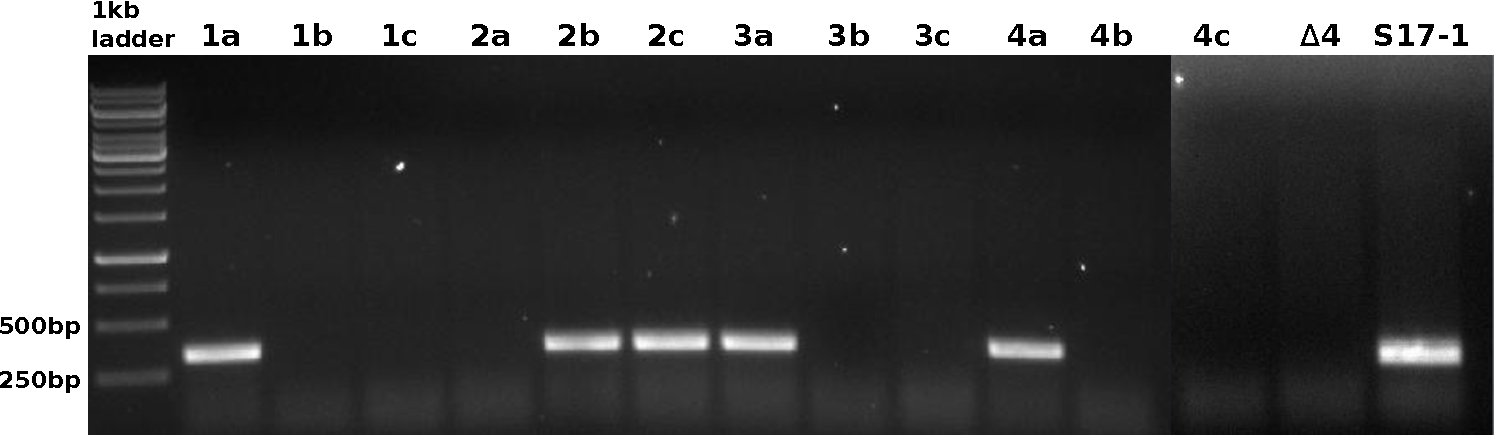
\includegraphics[width=0.9\textwidth,keepaspectratio=true]{graphics/delta4integrants.pdf}}
		\caption[\textit{P. fluorescens} $ \Delta $\textit{acp4} integrants validation.]{\textit{P. fluorescens} $ \Delta $\textit{acp4} integrants validation. Five out of twelve colonies as well as the positive control showed the presence of the ACP-K24a.}
		\label{fig:delta4integrands}
		\end{figure}	
	
	The previous steps validated the integration of the ACP-K24a into the \textit{P. fluorescens} $ \Delta $\textit{acp4} chromosome but it did not detect whether the integration happened at the correct position in the mupirocin cluster. In order to validate the integration of the ACP-K24a at the correct position another PCR was carried out on the five integrants. Primers were used that bind to positions outside the left and right arms, which had been previously designed by Dr. Anthony Haines.  \textit{P. fluorescens} NCIMB 10586 and \textit{P. fluorescens} $ \Delta $\textit{acp4} were used as the controls, with \textit{P. fluorescens} $ \Delta $\textit{acp4} expected to give a band equivalent in size to the five integrants since they have a single ACP at the branching position, whereas \textit{P. fluorescens} NCIMB 10586 would give a slightly bigger band because of the two tandem ACPs (Figure \ref{fig:delta4extended}). 

		\setlength\fboxsep{5pt}
		\setlength\fboxrule{1.5pt}
		\begin{figure}[htbp]
		\centering
		\fbox{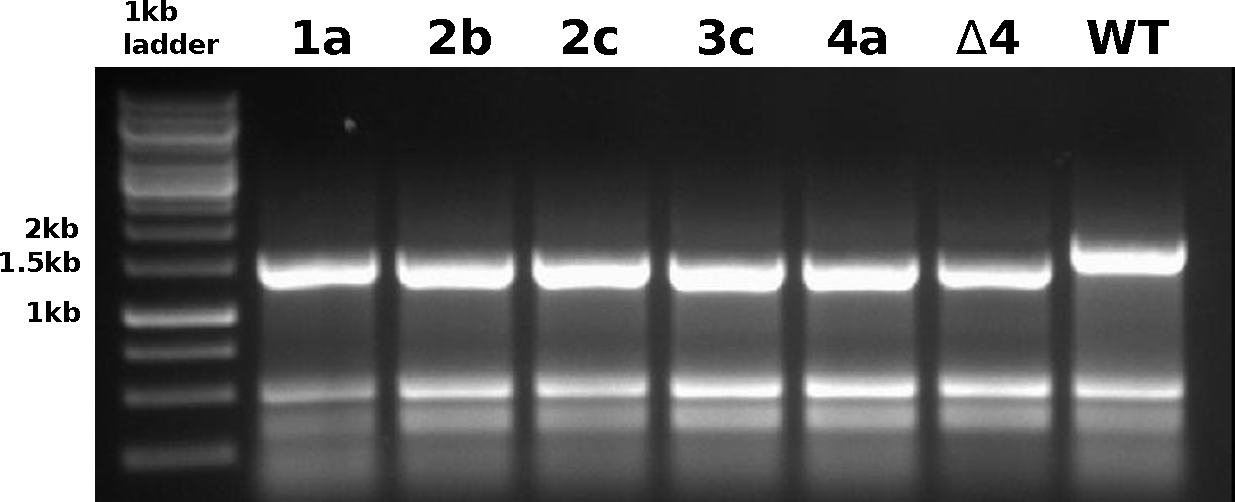
\includegraphics[width=0.9\textwidth,keepaspectratio=true]{graphics/delta4extended.pdf}}
		\caption[Five \textit{P. fluorescens} $ \Delta $\textit{acp4} integrants tested for correct location of ACP-K24a integration.]{Five \textit{P. fluorescens} $ \Delta $\textit{acp4} integrants tested for correct location of ACP-K24a integration.  The primers bind at locations outside the 500 bp arms thus the five integrants as well as $ \Delta $\textit{acp4}, have a band closer to 1.5 kb, which includes two arms of $ \approx $1 kb and an ACP of 331 nucleotides  while the wild type \textit{P. fluorescens} NCIMB 10586 which contains two ACPS and the linker region between them has slightly larger band. The primers also seem to mis-prime some where in the chromosome thus generating a smaller band of $ \approx $500 bp. }
		\label{fig:delta4extended}
		\end{figure}		

	The PCR product for the five integrants were further subjected to restriction digests using enzymes Blp I and Stu I. Blp I cuts approximately at the middle of the ACP-K24a but does not cut anywhere in ACP-mupA3a and Stu I cuts at the middle of the ACP-mupA3a as well as at the rear ends of the two arms. The restriction digest fragments were analysed with 1\% agarose gel electrophoresis, an uncut fragment was used as the control. Two samples verified by the restriction digestion of the PCR products were used for sequencing in the forward and reverse direction using the primers used in the previous step. Glycerol stocks of the two verified samples (two replicates for each i.e. $ \Delta $ 4-1a (tube 1 and 2) and 4-2b (tube 1 and 2)) were stored at -80\textcelsius.	
	
		\setlength\fboxsep{5pt}
		\setlength\fboxrule{1.5pt}
		\begin{figure}[htbp]
		\centering
		\fbox{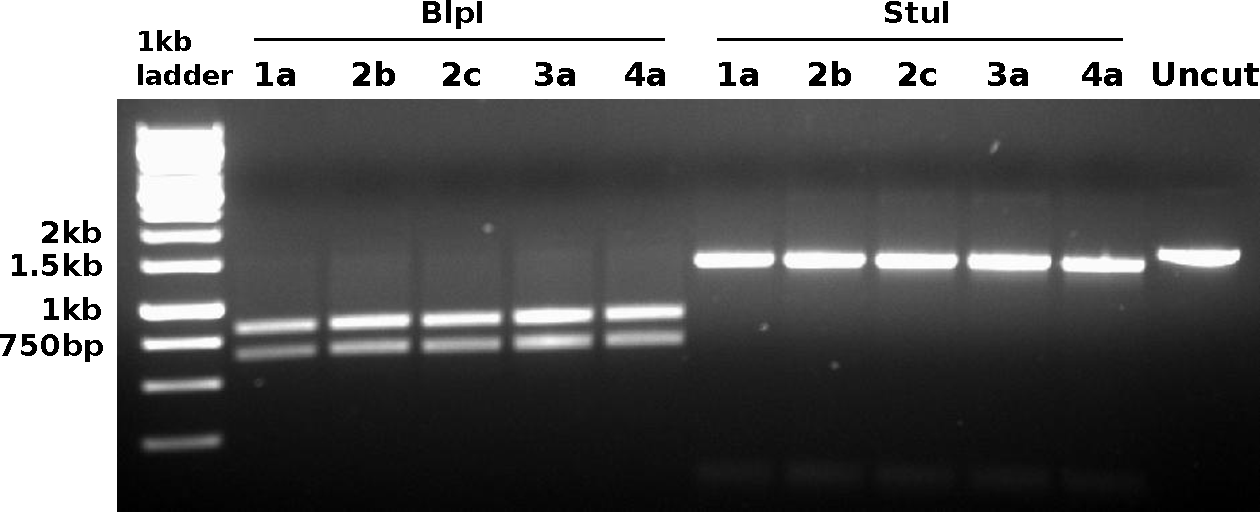
\includegraphics[width=0.9\textwidth,keepaspectratio=true]{graphics/delta4restriction.pdf}}
		\caption[Restriction digestion of the five \textit{P. fluorescens} $ \Delta $\textit{acp4} integrants.]{Restriction digestion of the five \textit{P. fluorescens} $ \Delta $\textit{acp4} integrants using restriction enzymes Blp I and Stu I. BlP I cuts approximately at the middle of the ACP-K24a and Stu I cuts approximately at the middle of the ACP-mupA3a as well as at the rear ends of the two arms. The first five wells shows ACP-K24a cut approximately at the middle whereas the next five shows the fragments which were cut only at the rear ends of the arms. The last well shows the actual size of the uncut DNA fragment.}
		\label{fig:delta4restriction}
		\end{figure}			
	
	For \textit{P. fluorescens} $ \Delta $\textit{mupH} trans-conjugants sucrose selection was performed following the same steps as for the \textit{P. fluorescens} $ \Delta $\textit{acp4} trans-conjugants. To validate the excisions and integrants, nine samples were subjected to PCR using the primers designed to bind at the region outside the two arms (Figure \ref{fig:deltahexcisants}), one of which was of the right size and was sequenced. Compared to the treatment of the \textit{P. fluorescens} $ \Delta $\textit{acp4} integrants, the steps of PCR with ACP-K24a specific primers and subsequent restriction digestions were excluded, because running a PCR using only the outer primers and sequencing the PCR products gave an equivalent result in fewer steps and less time. Glycerol stocks of the sample (two replicates i.e. $ \Delta $ H-6d (tube 1 and 2)) were stored at -80\textcelsius.
	
		\setlength\fboxsep{5pt}
		\setlength\fboxrule{1.5pt}
		\begin{figure}[htbp]
		\centering
		\fbox{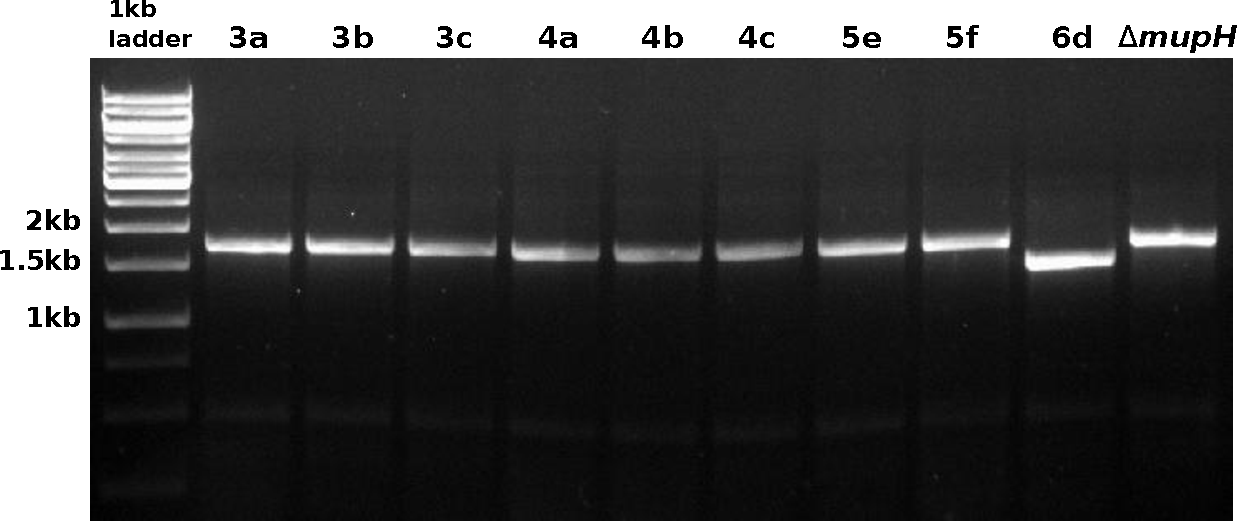
\includegraphics[width=0.9\textwidth,keepaspectratio=true]{graphics/deltahexcisants.pdf}}
		\caption[Nine \textit{P. fluorescens} $ \Delta $\textit{mupH} integrants tested for correct location of ACP-K24a integration.]{Nine \textit{P. fluorescens} $ \Delta $\textit{mupH} integrants tested for correct location of ACP-K24a integration. The primers used bind at the locations outside the 500 bp arms only one out of nine showed the band closer to 1.5 kb which includes two arms of $ \approx $1 kb and an ACP of 331 nucleotides while \textit{P. fluorescens} $ \Delta $\textit{mupH} which contains two ACPS and the linker region between them has slightly larger band along with all the other samples which probably reverted back to the wild type state during plasmid excision. The primers also seem to mis-prime some where in the chromosome thus generating a very faint band of $ \approx $500 bp.}
		\label{fig:deltahexcisants}
		\end{figure}

	\subsection{Overlay Bioassay to test for antibiotic production in the constructed strains}
	\label{sec:chap4bioassay}	
	To test the two hypothesises that the ACP-K24a from the kalimantacin cluster would not work with MupH but will work with BatC, three previously prepared pJH10 plasmids containing \textit{mupH}, \textit{batC} or the \textit{batC} L218M mutant were expressed \textit{in trans} in the newly constructed \textit{P. fluorescens} $ \Delta $H-6d strain. One pJH10 plasmid containing \textit{batC} was also expressed \textit{in trans} in the newly constructed  \textit{P. fluorescens} $ \Delta $4-1a strain (see details in section \ref{sec:bioassay}). Since, $ \Delta $H-6d strain lacks \textit{mupH} in the HCS cassette, the \textit{in trans} expression of any of \textit{mupH}, \textit{batC} or \textit{batC} L218M mutant in this strain would test for a functional interaction with ACP-K24a. It was thought that the interaction of ACP-K24a with \textit{mupH}, whether \textit{in trans} or on the chromosome (as in  $ \Delta $4-1a strain), would be unfavourable. On the other hand the interaction of ACP-K24a with \textit{batC} \textit{in trans} should be favourable in the $ \Delta $H-6d strain and it should also have some favourable effect in $ \Delta $4-1a strain, since the \textit{batC} expressed \textit{in trans} would compete with the chromosomal \textit{mupH} to interact with ACP-K24a. The three plasmids that were previously transformed into the \textit{E. coli} S17-1 strain were used for the conjugal transfer of the plasmids into \textit{P. fluorescens} $ \Delta $H-6d and 4-1a cells. The trans-conjugants were purified over minimal media to get rid of the \textit{E. coli} S17-1 strain and were validated by plasmid extraction and gel electrophoresis.
	
	For the bioassay three replicates of each strain were spotted and the antibiotic efficacy was measured as the diameter of the clearance zone, excluding the size of the central disc. The average of two diameters was calculated and the standard deviation between the averages of the three replicates were plotted as error bars in a bar graph (Figure \ref{fig:bioassaygraph}). A bioassay for each sample was carried out with and without IPTG induction.
	
		\setlength\fboxsep{5pt}
		\setlength\fboxrule{1.5pt}
		\begin{figure}[htbp]
		\centering
		\fbox{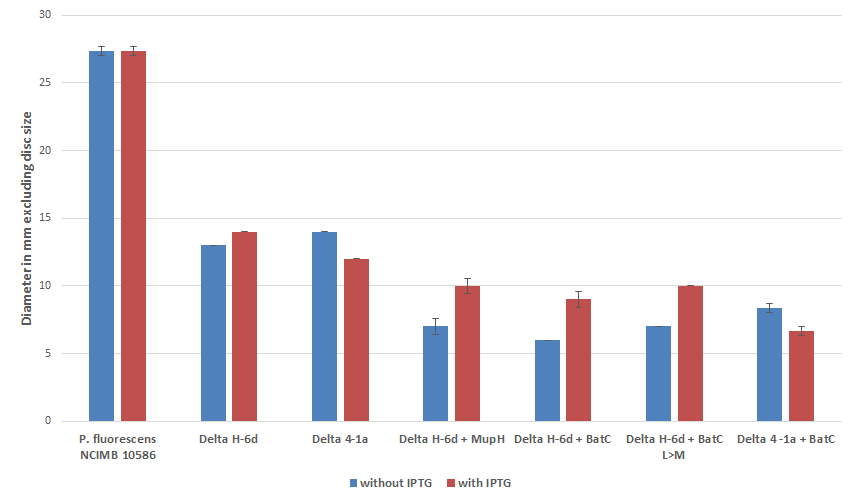
\includegraphics[width=0.9\textwidth,keepaspectratio=true]{graphics/bioassaygraph.png}}
		\caption[Bioassay results for \textit{in trans} expression of \textit{mupH}, \textit{batC} or the \textit{batC} L218M mutant.]{Bioassay results for \textit{in trans} expression of \textit{mupH}, \textit{batC} or the \textit{batC} L218M mutant with and without IPTG induction. \textit{P. fluorescens} NCIMB 10586 is the wild type mupirocin producer, $ \Delta $H-6d and $ \Delta $4-1a carry ACP-K24a in place of mupA3a\&b-ACP in the mupirocin cluster. $ \Delta $H-6d lacks chromosomal \textit{mupH}. \textit{mupH}, \textit{batC} and \textit{batC} L218M were the genes on pJH10 plasmid expressed \textit{in trans}. Error bars represents the standard deviation of three replicates with two diameters measured per strain.}
		\label{fig:bioassaygraph}
		\end{figure}	
	
	The bioassay results showed the $ \Delta $4-1a strain had a diameter for the clearance zone that was 50 \% of WT. A similar change was  observed in the  $ \Delta $H-6d strain which does not contain chromosomal \textit{mupH} in the HCS cassette. Upon expressing \textit{batC} \textit{in trans} in the $ \Delta $4-1a strain the clearance zone diameter was found to be almost half of that of the $ \Delta $4-1a strain without \textit{batC}, both with and without IPTG induction. Expressing \textit{mupH} \textit{in trans} in the $ \Delta $H-6d strain gave a clearance zone slightly smaller with IPTG and much smaller without IPTG, as compared to the $ \Delta $4-1a strain. The clearance zone of the  $ \Delta $H-6d strain with \textit{in trans} expression of \textit{batC} did not differ greatly from  $ \Delta $H-6d with \textit{mupH} \textit{in trans}. A similar clearance zone was also observed for $ \Delta $H-6d with \textit{batC} L218M expressed \textit{in trans}. Figure \ref{fig:bioassayplates} shows the plate bioassay for one of the replicates of each sample with and without IPTG induction.

	
		\setlength\fboxsep{5pt}
		\setlength\fboxrule{1.5pt}
		\begin{sidewaysfigure}[htbp]
		\centering
		\fbox{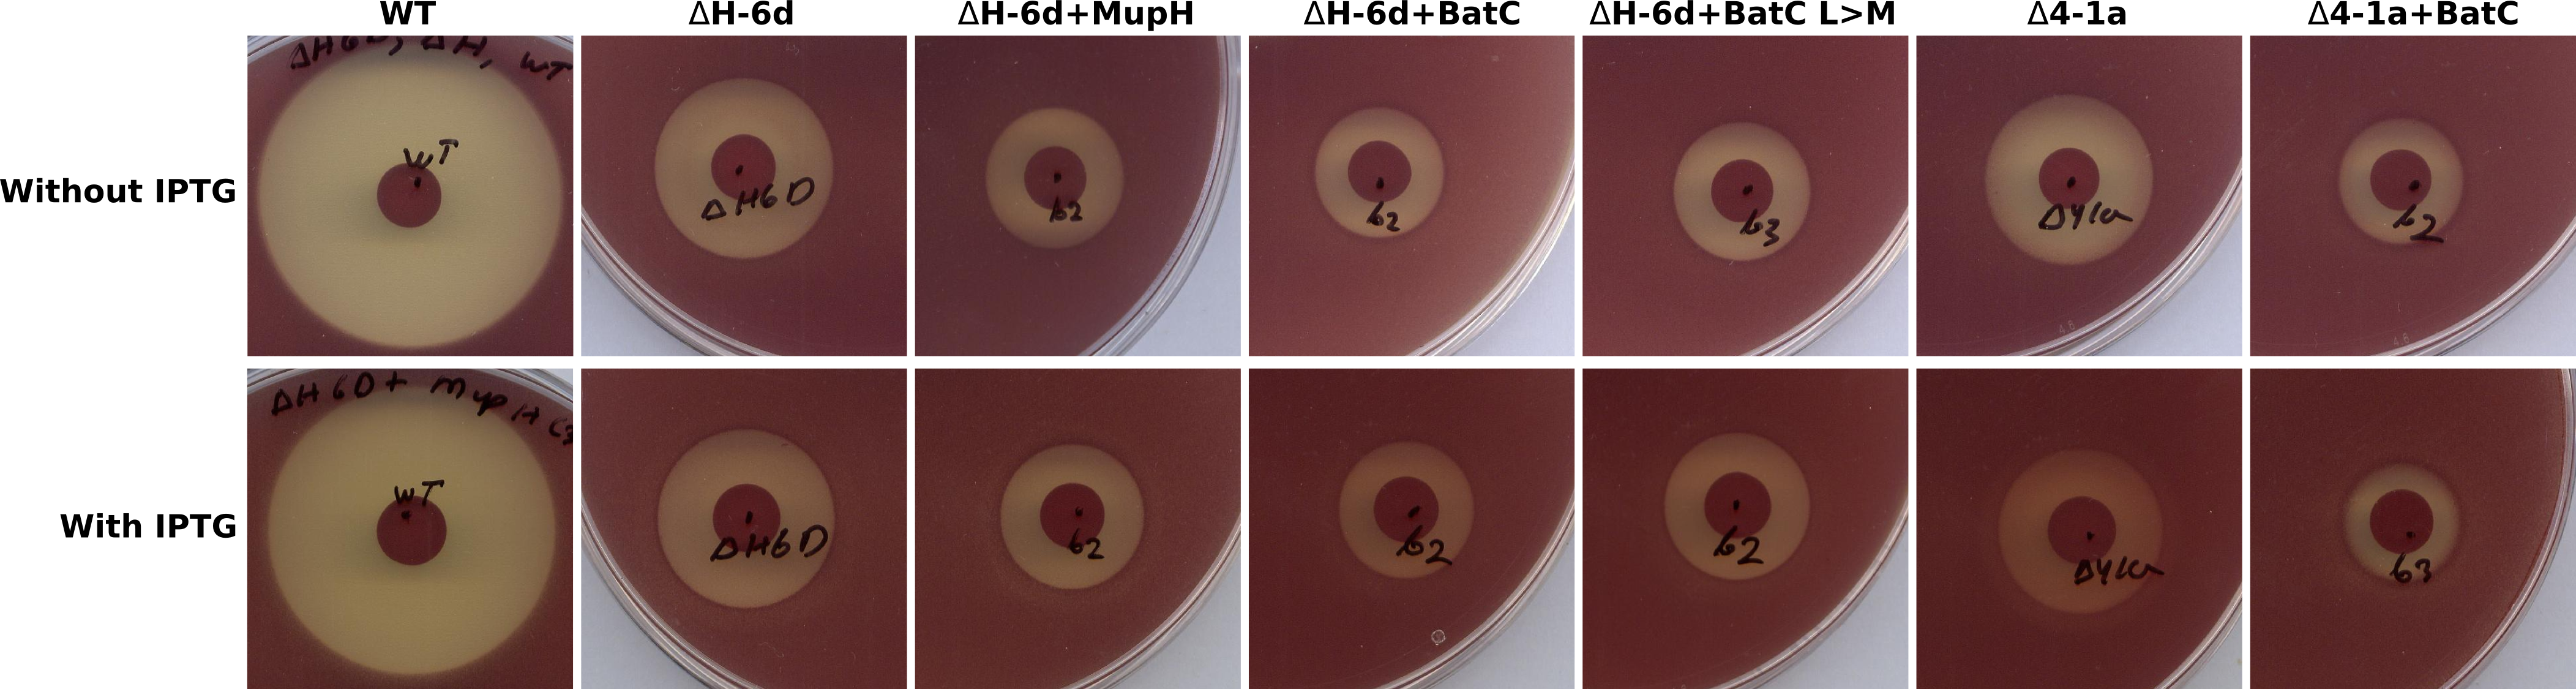
\includegraphics[width=0.9\textwidth,keepaspectratio=true]{graphics/bioassayplates.png}}
		\caption[Plate bioassay for one of the replicates of each sample with and without IPTG induction.]{Plate bioassay for one of the replicates of each sample with and without IPTG induction. WT is the \textit{P. fluorescens} NCIMB 10586 wild type mupirocin producer, $ \Delta $H-6d and $ \Delta $4-1a carry ACP-K24a in place of mupA3a\&b-ACP in the mupirocin cluster. $ \Delta $H-6d lacks chromosomal \textit{mupH}. \textit{mupH}, \textit{batC} and \textit{batC} L218M were the genes on pJH10 plasmid expressed \textit{in trans}.}
		\label{fig:bioassayplates}
		\end{sidewaysfigure}		
\newpage
	\subsection{HPLC analysis for \textit{in trans} expression of MupH, BatC and BatC L218M mutant}
	\label{sec:chap4HPLC}
	In order to detect pseudomonic acids produced by the \textit{in trans} expression of \textit{mupH}, \textit{batC} or \textit{batC} L218M in \textit{P. fluorescens} $ \Delta $H-6d and $ \Delta $4-1a strains, HPCL were performed. \textit{P. fluorescens} NCIMB 10586 and \textit{P. fluorescens}  $ \Delta $H-6d and $ \Delta $4-1a with blank pJH10 plasmid were used as controls (see methods section \ref{sec:hplc}). The chromatograms plotted in Figures \ref{fig:hplcwt} to \ref{fig:hplcdelta4batc} were zoomed in on the 5 min to 30 min retention time. Figure \ref{fig:hplcwt} shows a representative chromatogram of the elution profile of pseudomonic acid A produced by \textit{P. fluorescens} NCIMB 10586. For the three replicates the average retention time and peak area were 20:21 min and 48273600 respectively. Figures \ref{fig:hplcdeltahphj10} to \ref{fig:hplcdeltahbatclm} show the chromatograms of the elution profile for the products produced by \textit{P. fluorescens} $ \Delta $H-6d strain , and Figures \ref{fig:hplcdelta41a} to \ref{fig:hplcdelta4batc} show the chromatograms of the elution profile for the products produced by \textit{P. fluorescens} $ \Delta $4-1a strain. No observable peak was detected for any of the known pseudomonic acids in any of these figures, however, a distinct peak for an unknown product was observed at around 17:57 min retention time for all \textit{P. fluorescens} $ \Delta $4-1a strain (Figure \ref{fig:hplcdelta41a} to \ref{fig:hplcdelta4batc}). 
	
		\setlength\fboxsep{5pt}
		\setlength\fboxrule{1.5pt}
		\begin{figure}[htbp]
		\centering
		\fbox{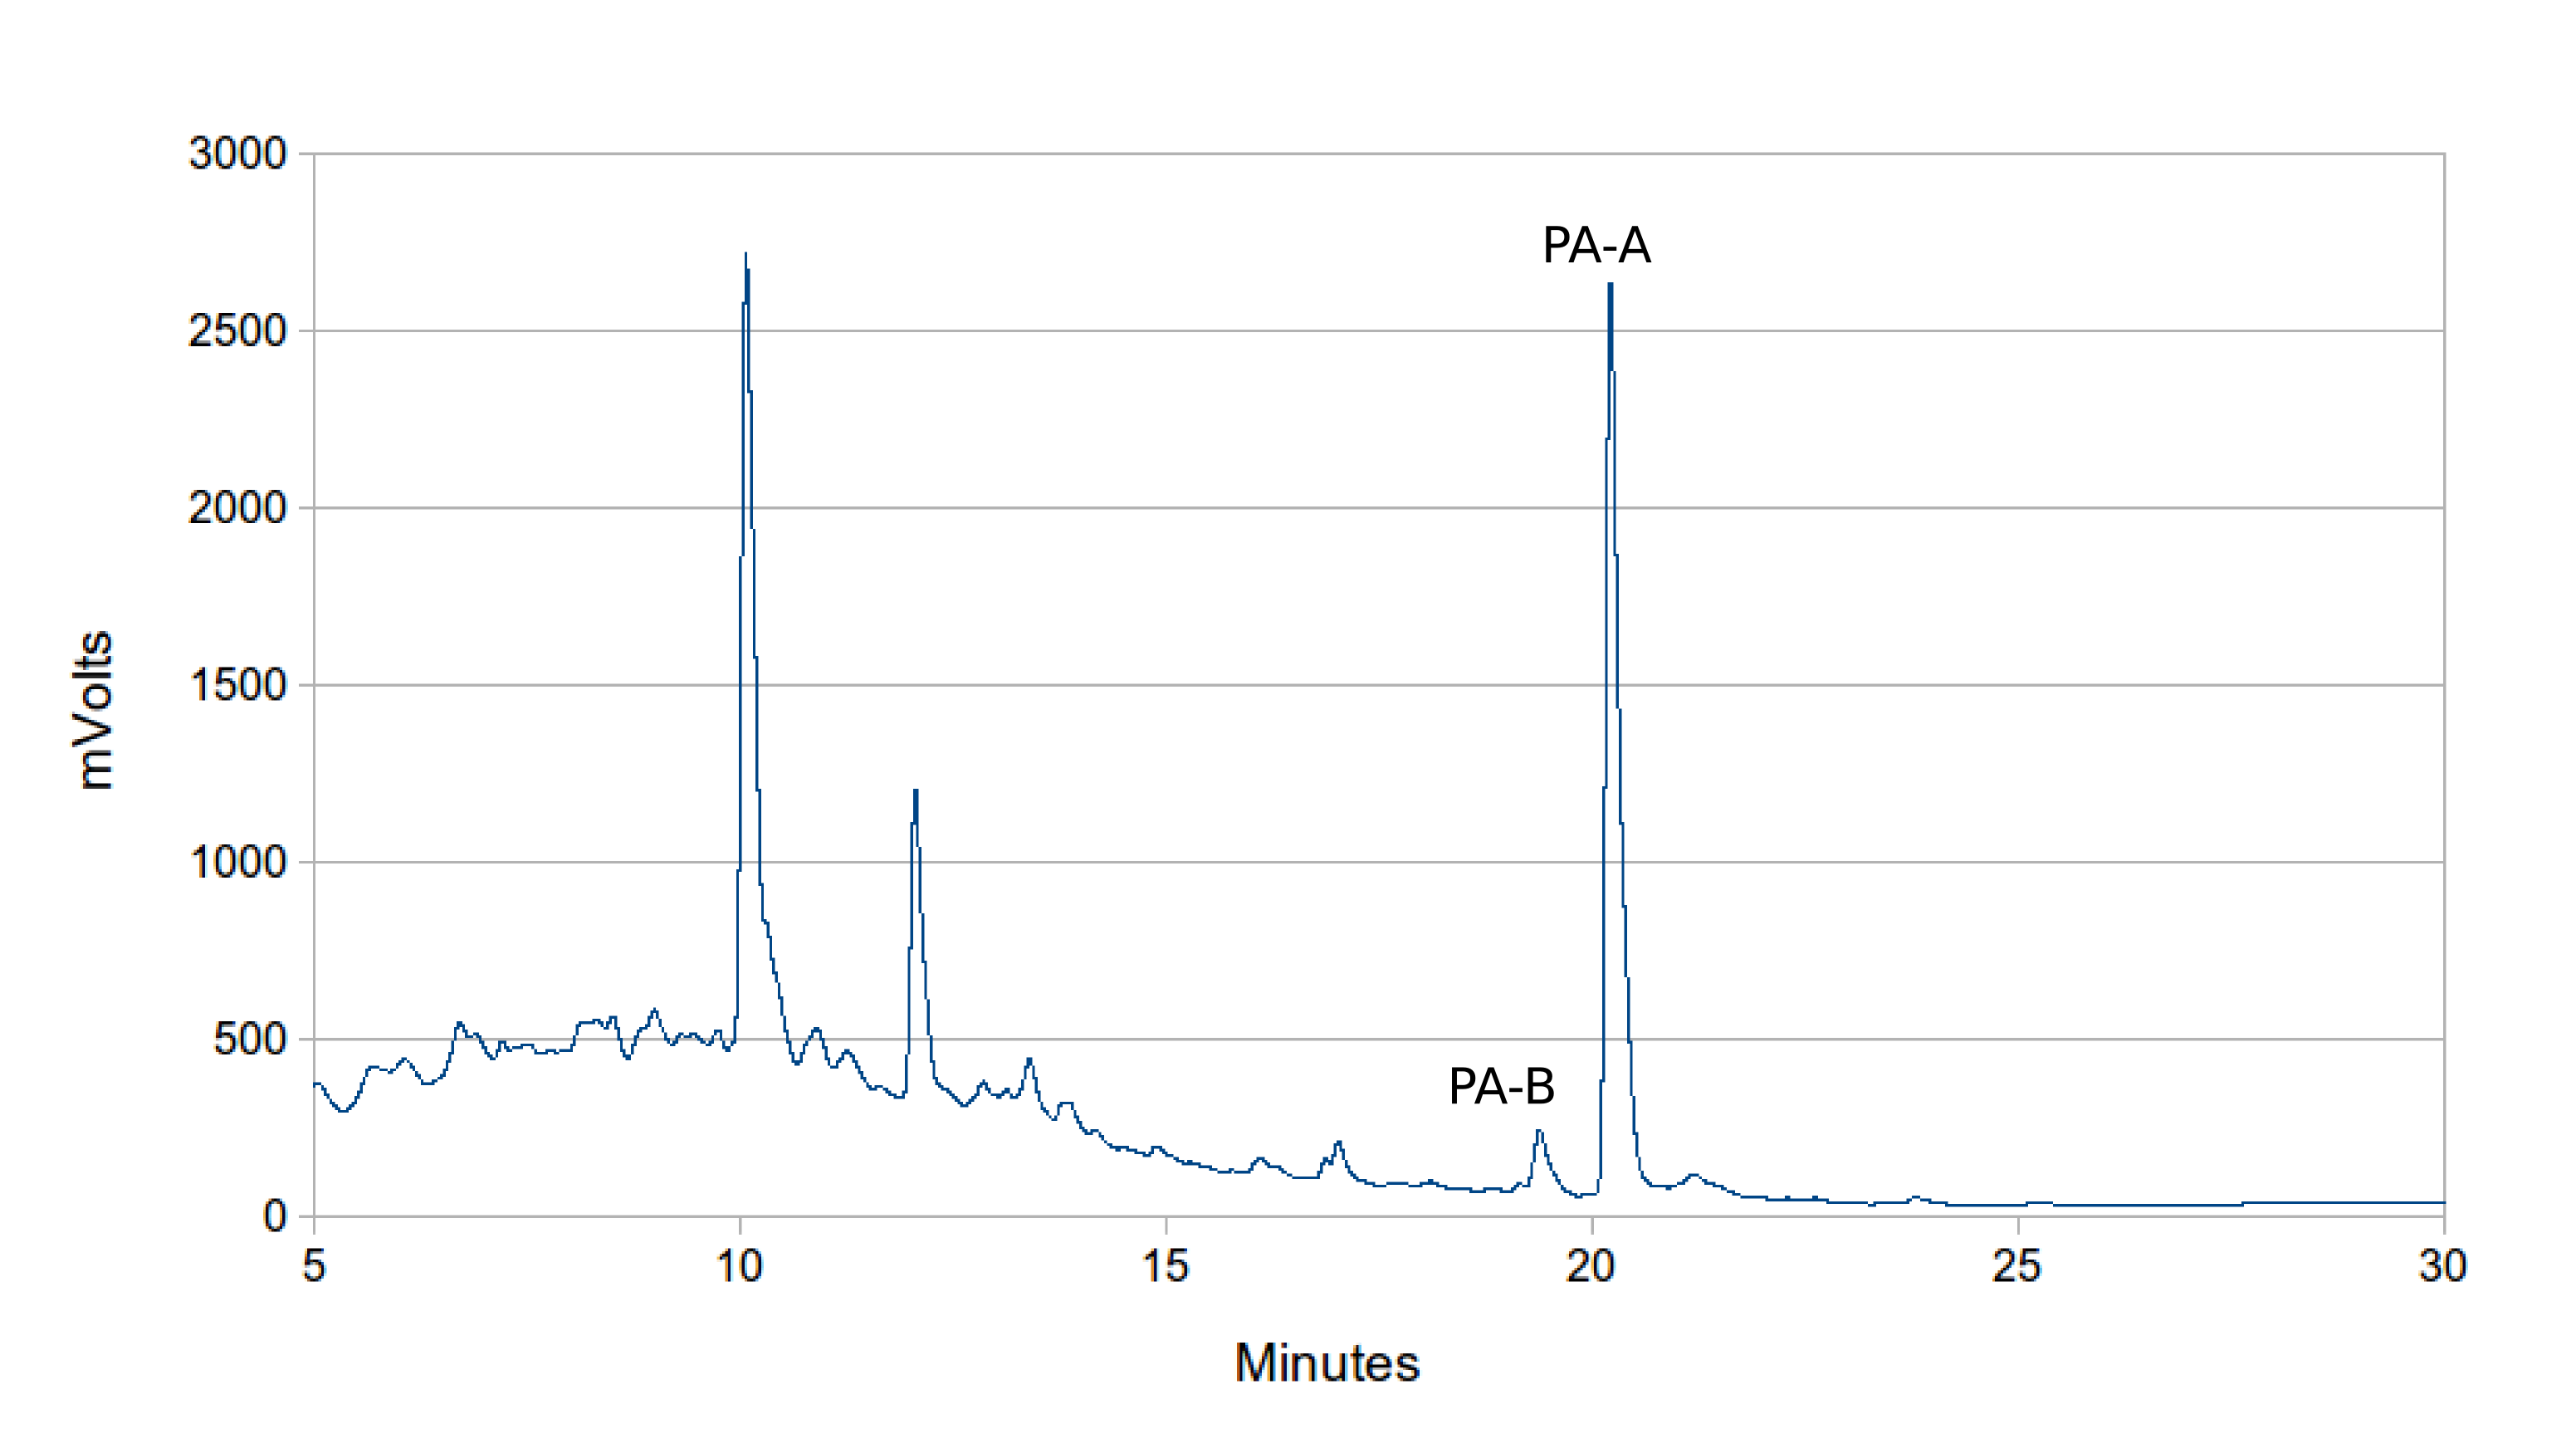
\includegraphics[width=0.9\textwidth,keepaspectratio=true]{graphics/wt.png}}
		\caption[HPLC trace for \textit{P. fluorescens} NCIMB 10586. ]{HPLC trace for \textit{P. fluorescens} NCIMB 10586.}
		\label{fig:hplcwt}
		\end{figure}

		\setlength\fboxsep{5pt}
		\setlength\fboxrule{1.5pt}
		\begin{figure}[htbp]
		\centering
		\fbox{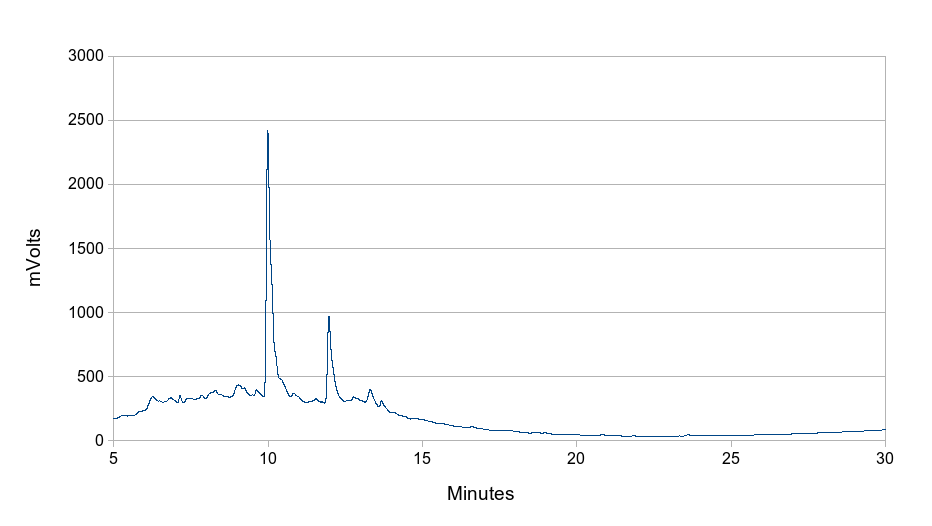
\includegraphics[width=0.9\textwidth,keepaspectratio=true]{graphics/deltahpjh102.png}}
		\caption[HPLC trace for \textit{P. fluorescens} $ \Delta $H-6d strain with blank pJH10 plasmid. ]{HPLC trace for \textit{P. fluorescens} $ \Delta $H-6d strain with blank pJH10 plasmid.}
		\label{fig:hplcdeltahphj10}
		\end{figure}

		\setlength\fboxsep{5pt}
		\setlength\fboxrule{1.5pt}
		\begin{figure}[htbp]
		\centering
		\fbox{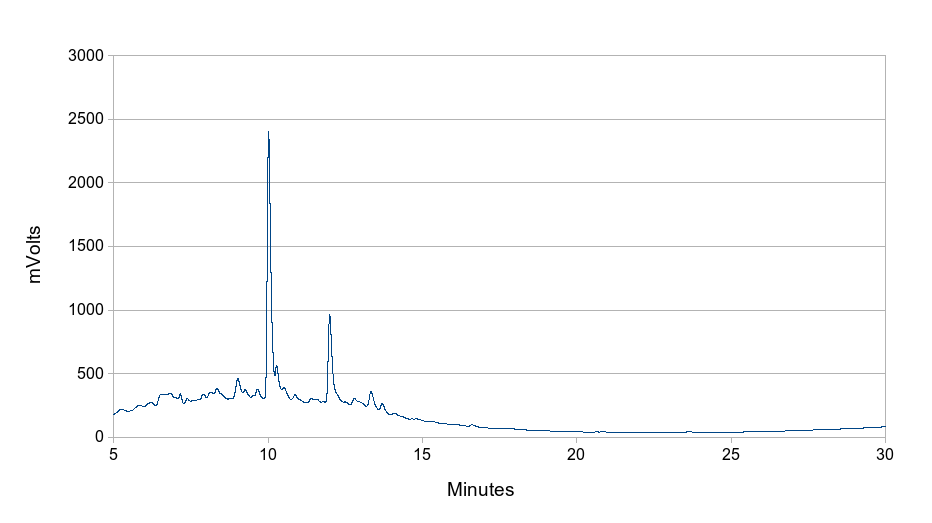
\includegraphics[width=0.9\textwidth,keepaspectratio=true]{graphics/deltahmuph2.png}}
		\caption[HPLC trace for \textit{P. fluorescens} $ \Delta $H-6d strain with \textit{mupH} expressed \textit{in trans}. ]{HPLC trace for \textit{P. fluorescens} $ \Delta $H-6d strain with \textit{mupH} expressed \textit{in trans}.}
		\label{fig:hplcdeltahmuph}
		\end{figure}			

		\setlength\fboxsep{5pt}
		\setlength\fboxrule{1.5pt}
		\begin{figure}[htbp]
		\centering
		\fbox{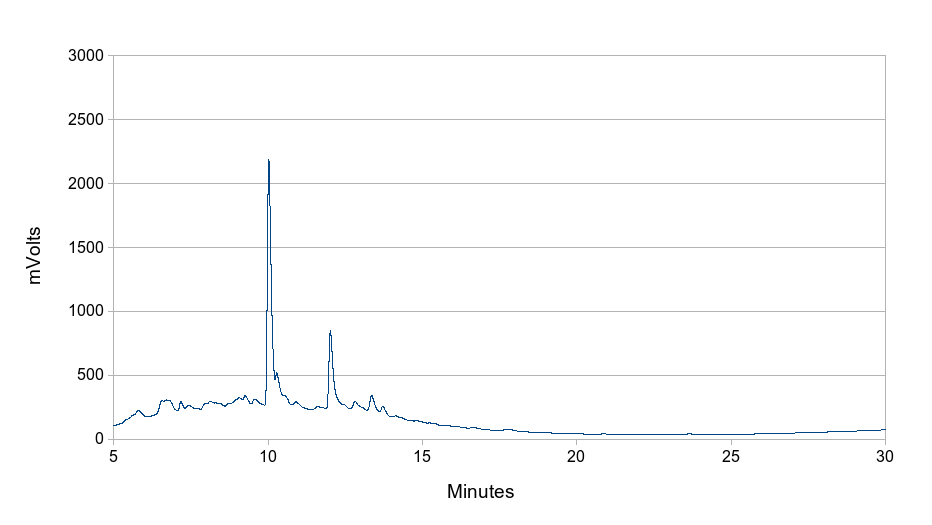
\includegraphics[width=0.9\textwidth,keepaspectratio=true]{graphics/deltahbatc2.png}}
		\caption[HPLC trace for \textit{P. fluorescens} $ \Delta $H-6d strain with \textit{batC} expressed \textit{in trans}. ]{HPLC trace for \textit{P. fluorescens} $ \Delta $H-6d strain with \textit{batC} expressed \textit{in trans}.}
		\label{fig:hplcdeltahbatc}
		\end{figure}

		\setlength\fboxsep{5pt}
		\setlength\fboxrule{1.5pt}
		\begin{figure}[htbp]
		\centering
		\fbox{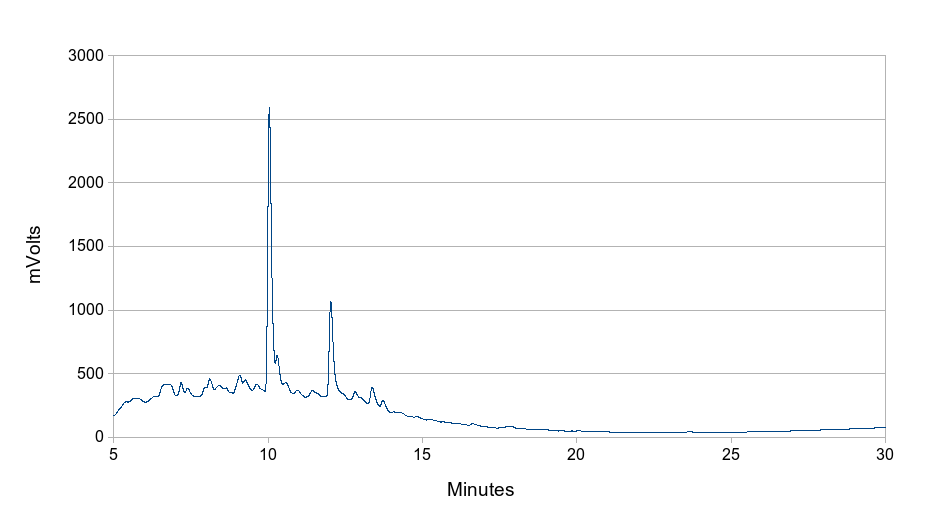
\includegraphics[width=0.9\textwidth,keepaspectratio=true]{graphics/deltahbatcLM2.png}}
		\caption[HPLC trace for \textit{P. fluorescens} $ \Delta $H-6d strain with \textit{batC} L to M mutant expressed \textit{in trans}. ]{HPLC trace for \textit{P. fluorescens} $ \Delta $H-6d strain with \textit{batC} L to M mutant expressed \textit{in trans}.}
		\label{fig:hplcdeltahbatclm}
		\end{figure}					

		\setlength\fboxsep{5pt}
		\setlength\fboxrule{1.5pt}
		\begin{figure}[htbp]
		\centering
		\fbox{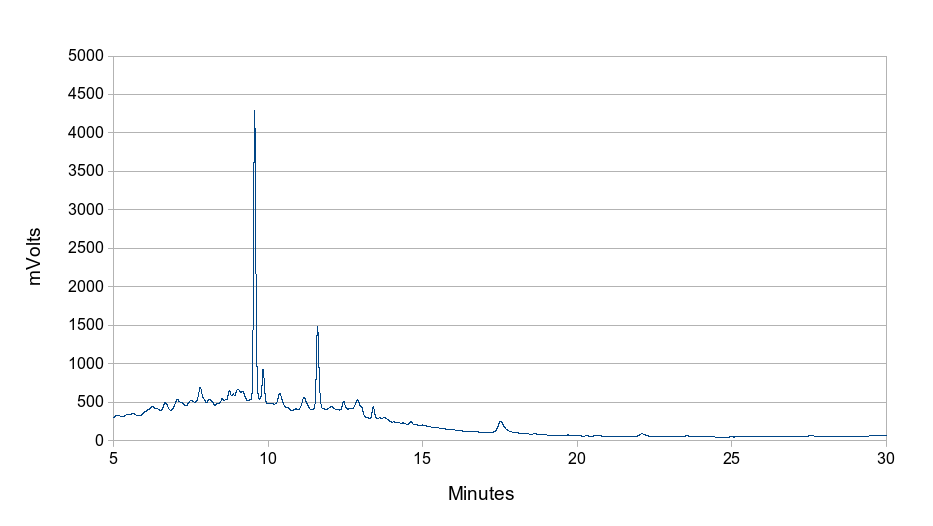
\includegraphics[width=0.9\textwidth,keepaspectratio=true]{graphics/delta41a3.png}}
		\caption[HPLC trace for \textit{P. fluorescens} $ \Delta $4-1a strain. ]{HPLC trace for \textit{P. fluorescens} $ \Delta $4-1a strain}
		\label{fig:hplcdelta41a}
		\end{figure}	

		\setlength\fboxsep{5pt}
		\setlength\fboxrule{1.5pt}
		\begin{figure}[htbp]
		\centering
		\fbox{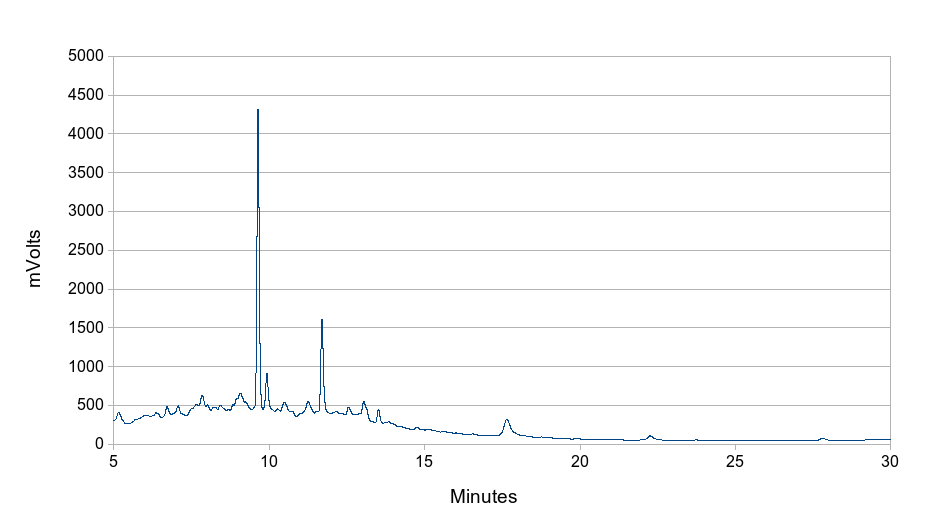
\includegraphics[width=0.9\textwidth,keepaspectratio=true]{graphics/delta4pjh102.png}}
		\caption[HPLC trace for \textit{P. fluorescens} $ \Delta $4-1a strain with blank pJH10 plasmid. ]{HPLC trace for \textit{P. fluorescens} $ \Delta $4-1a strain with blank pJH10 plasmid.}
		\label{fig:hplcdelta4phj10}
		\end{figure}

		\setlength\fboxsep{5pt}
		\setlength\fboxrule{1.5pt}
		\begin{figure}[htbp]
		\centering
		\fbox{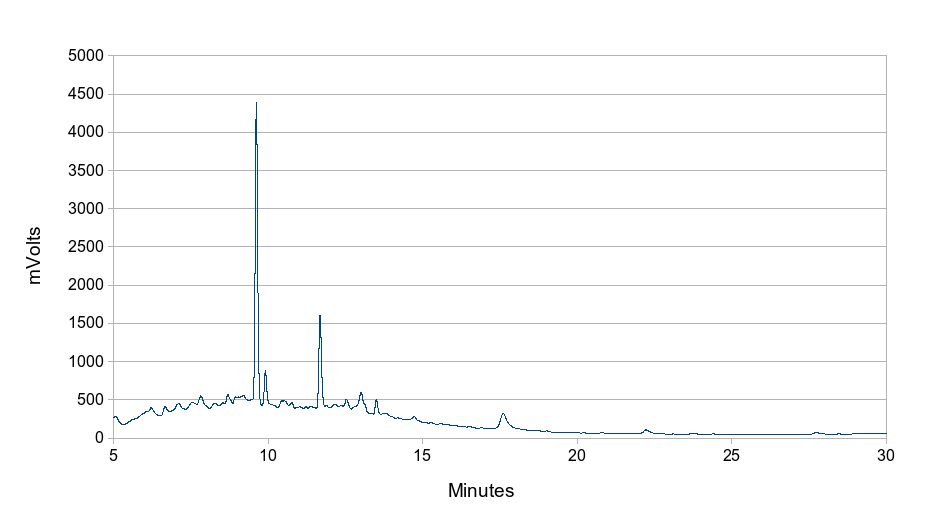
\includegraphics[width=0.9\textwidth,keepaspectratio=true]{graphics/delta4batc1.png}}
		\caption[HPLC trace for \textit{P. fluorescens}  $ \Delta $4-1a strain with \textit{batC} expressed \textit{in trans}. ]{HPLC trace for \textit{P. fluorescens}  $ \Delta $4-1a strain with \textit{batC} expressed \textit{in trans}.}
		\label{fig:hplcdelta4batc}
		\end{figure}

\newpage		

	\subsection{Molecular dynamics simulation of ACP-mupA3a+MupH complex}
	\label{sec:chap4acpmuphmd}
	Molecular dynamics simulations were carried out on the ACP-mupA3a + MupH complex obtained from HADDOCK (see section \ref{sec:MupHACPInteraction}). The starting conformation was setup to mimic the condensation stage in the HMG-CoA reaction mechanism (see Figure \ref{fig:HMGCO-Areact}), with monic acid attached to the phosphopantetheine arm of ACP-mupA3a and acetyl attached to C115 of MupH, to mimic the \bet-branching step. Three independent simulations were run for 50 ns each. Coordinate files were extracted at every 4 ns from the trajectory and residues in ACP-mupA3a that were within 5 \AA \ distance of M219 (MupH) were selected. Residue R30 and L32 were found to be highlighted in all the frames whereas Y62 and P65 were highlighted in most of the frames (Figure \ref{fig:lmsimulation}).

		\setlength\fboxsep{5pt}
		\setlength\fboxrule{1.5pt}
		\begin{figure}[htbp]
		\centering
		\fbox{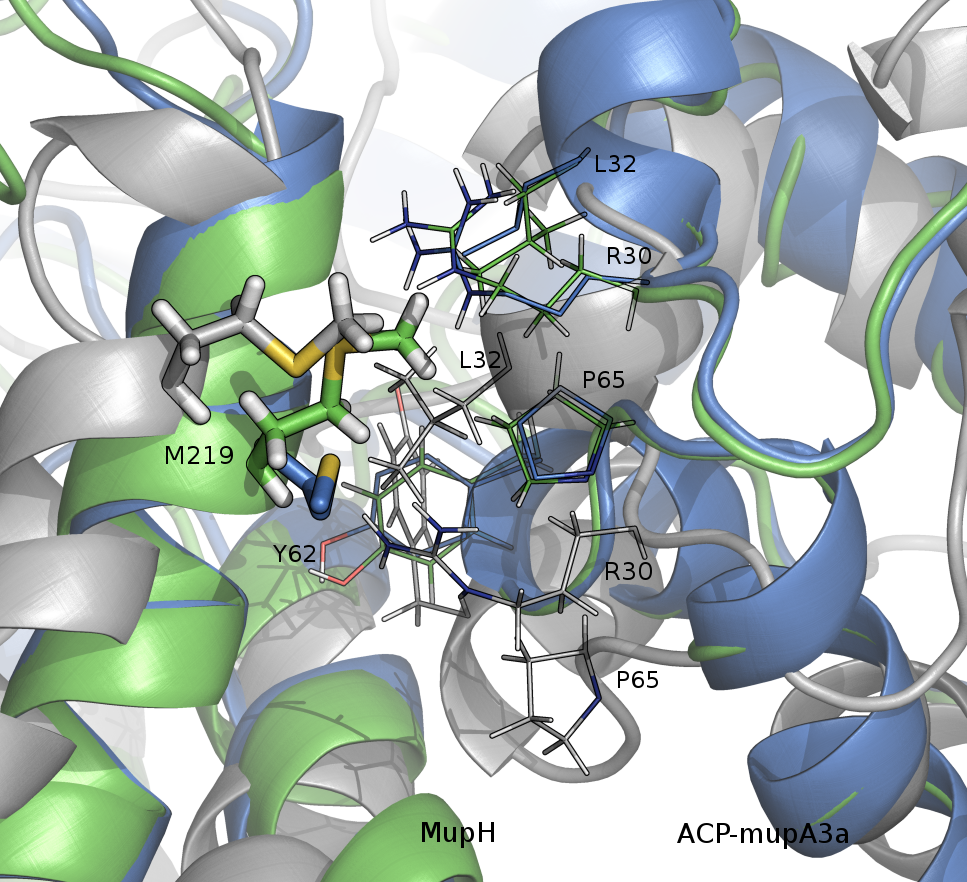
\includegraphics[width=0.9\textwidth,keepaspectratio=true]{graphics/lmsimulation.png}}
		\caption[ACP-mupA3a + MupH complex interface refined by molecular dynamics simulation.]{ACP-mupA3a + MupH complex interface refined by molecular dynamics simulation. Blue: complex I of the ACP-mupA3a + MupH docked complex; Green: first frame (10 ps) of the ACP-mupA3a + MupH simulation; Grey: last frame (50 ns)  of of the ACP-mupA3a + MupH simulation. R30 and L32 were highlighted within 5 \AA of M219 in all the frames whereas Y62 and P65 were mostly highlighted.}
		\label{fig:lmsimulation}
		\end{figure}	
	
	Based on this observation it was proposed that either these positions or their neighbours were responsible for the ACP recognition specificity associated with position M219 of MupH and its homologues. To test this hypothesis and plan mutagenesis experiments Dr. Anthony Haines segregated the \bet-branching ACPs from well characterised clusters into two groups based on whether their cognate HCS protein carried a methionine or a leucine. Figure \ref{fig:lmalignment} shows the alignment of the two groups. Figure \ref{fig:lmlogo} shows sequence logos built from these alignments. Neither the R30 or the  L32 position equivalent or their neighbouring positions were differentially conserved in one set compared to the other.

		\setlength\fboxsep{5pt}
		\setlength\fboxrule{1.5pt}
		\begin{figure}[htbp]
		\centering
		\fbox{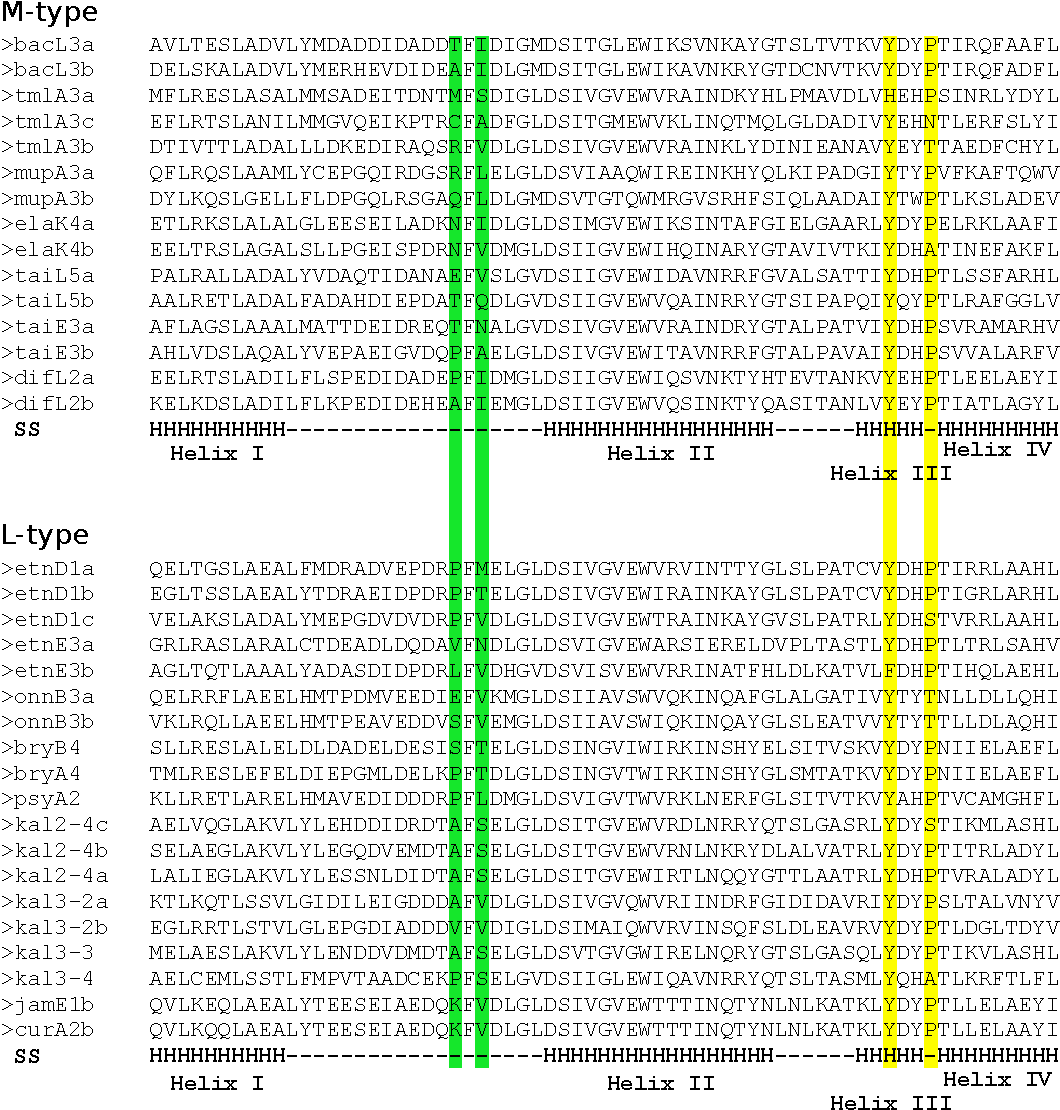
\includegraphics[width=0.9\textwidth,keepaspectratio=true]{graphics/lmalignment.pdf}}
		\caption[Sequence alignment of the \bet-branching ACPs segregated into two groups based on their cognate HCS protein.]{Sequence alignment of the \bet-branching ACPs segregated into two groups based on their cognate HCS protein. Green/Yellow: residue position which was always/mostly highlighted with 5 \AA \ of M219 in all the frames of molecular dynamics simulation respectively.}
		\label{fig:lmalignment}
		\end{figure}		

		\setlength\fboxsep{5pt}
		\setlength\fboxrule{1.5pt}
		\begin{figure}[htbp]
		\centering
		\fbox{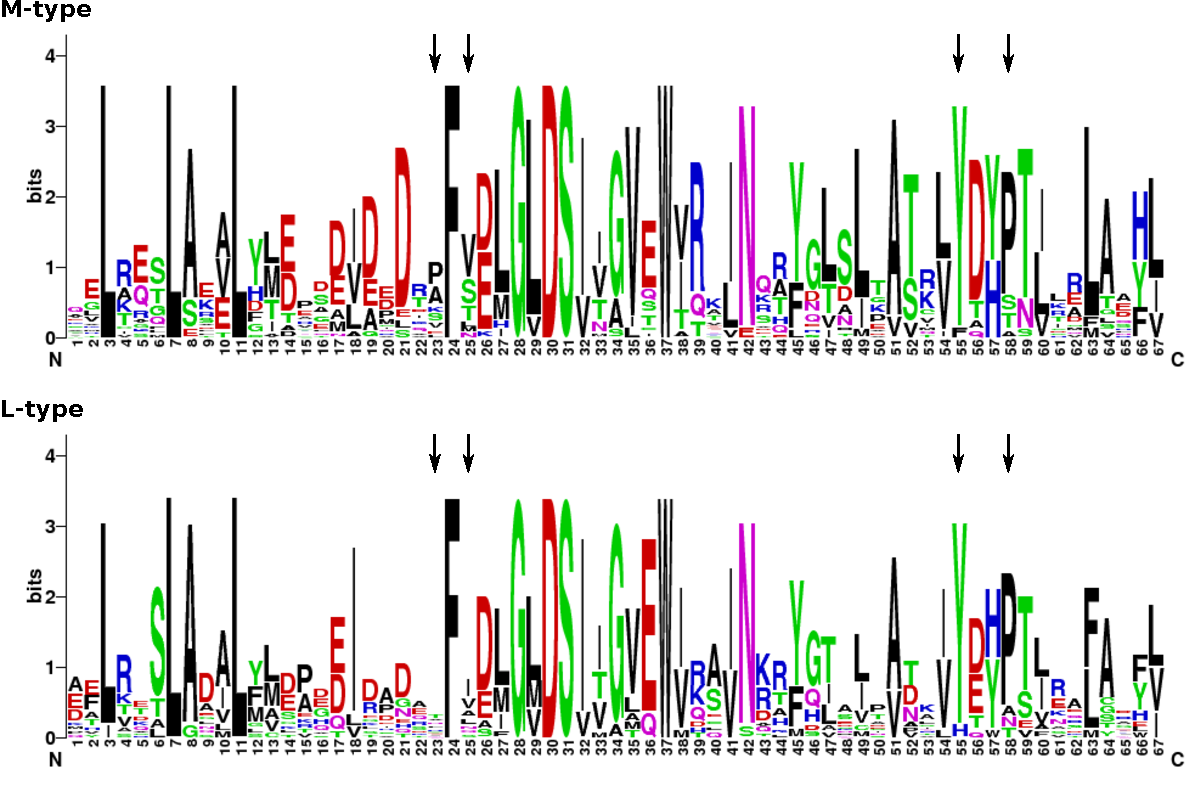
\includegraphics[width=0.9\textwidth,keepaspectratio=true]{graphics/lmlogo.pdf}}
		\caption[Sequence logo built on the alignment of the \bet-branching ACPs segregated into two groups based on their cognate HCS protein.]{Sequence logo built on the alignment of the \bet-branching ACPs segregated into two groups based on their cognate HCS protein. Arrows shows the residue positions which were always/mostly highlighted with 5 \AA \ of M219 in all the frames of molecular dynamics simulation.}
		\label{fig:lmlogo}
		\end{figure}		

\newpage

\section{Discussion}
\label{sec:chap4discussion}
These experiments were designed to gain a deeper understanding of the interaction of \bet-branching ACPs with the HCS proteins by replacing the mupirocin \bet-branching ACPs with one from the kalimantacin cluster. It was proposed in the previous chapter that \bet-branching is a phenomenon that is dependent on the recognition specificity of a subclass of ACPs by proteins in the HCS cassette and it was demonstrated that this subclass required a conserved tryptophan in the core of the ACP, six residues downstream of the catalytic serine. This tryptophan packing in the core of the ACP appears to allow helix III to be presented at an angle which facilitates its interaction with MupH. It was also found that a residue at the position 219 on MupH alternates between a methionine and a leucine in the MupH orthologues. Moreover MupH and TmlH, which complement a $ \Delta $MupH strain, have methionine, whereas BatC, which doesn't complement $ \Delta $MupH, has leucine. Mutating this leucine in BatC into methionine does allow complementation of $ \Delta $MupH. This gain of function experiment, along with other mutations, supported the computationally predicted ACP-MupH complex and suggested the possibility of engineering \bet-branching into different positions in PKS pathways. It also suggested that there exists an ACP-HCS subtype pairwise specificity. Pairwise specificity is indeed observed in the myxovirescin system, where the two HCS cassettes interact with different cognate ACPs,  without apparent cross talk.

The next obvious question was to test whether the \bet-branching ACPs from the kalimantacin cluster can complement the \bet-branching ACPs in the mupirocin cluster. It was hypothesised that, as \textit{batC} was very poor at complementing $ \Delta $\textit{mupH} mutant in the mupirocin cluster, ACP-K24a will not complement \bet-branching ACPs in the mupirocin cluster. However, either by expressing \textit{batC} \textit{in trans} or upon mutating ACP-K24a to favourably interact with MupH there should be an increase in the production of pseudomonic acids. To test this hypothesis, \bet-branching ACP-mupA3a and ACP-mupA3ab in the \textit{P. fluorescens}  $ \Delta $\textit{acp4} and  $ \Delta $\textit{mupH} strains respectively were replaced with ACP-K24a from the kalimantacin cluster. Suicide mutagenesis lead to the formation of the \textit{P. fluorescens} $ \Delta $H-6d strain which lacked \textit{mupH} and \textit{acp-mupA3ab} on the chromosome but had \textit{acp-K24a} incorporated into the chromosome, and the \textit{P. fluorescens} $ \Delta $4-1a strain which had \textit{mupH} and \textit{acp-K24a} on the chromosome, but no \textit{acp-mupA3ab}. Bioassay and HPLC analysis was carried out by expressing \textit{mupH}, \textit{batC} or \textit{batC} L218M mutant \textit{in trans} in the $ \Delta $H-6d strain and BatC \textit{in trans} in the $ \Delta $4-1a strain.

Bioassay results showed the $ \Delta $4-1a strain had a diameter for the clearance zone that was 50\% of WT, this observation was consistent with the original hypothesis that there would be either no or an unfavourable interaction between ACP-K24a and MupH. However, a similar drop was also observed in the  $ \Delta $H-6d strain which does not contain chromosomal \textit{mupH} in the HCS cassette. It was also thought that \textit{in trans }expression of \textit{batC} in $ \Delta $4-1a strain might increase the antibiotic production as BatC will compete with MupH for ACP-K24a and would make a more favourable interaction. However, the clearance zone was found to have almost half the diameter of that of the $ \Delta $4-1a strain without \textit{batC} expressed \textit{in trans}, both with and without IPTG induction. $ \Delta $H-6d with \textit{in trans} expression of \textit{mupH} should have given a similar clearance zone to that of the $ \Delta $4-1a strain as the only difference was that \textit{mupH} is on the pJH10 plasmid in the former and on the chromosome in the latter. However, the clearance zone was much smaller without IPTG and slightly smaller with IPTG, as compared to the $ \Delta $4-1a strain. $ \Delta $H-6d strain with \textit{in trans} expression of BatC, which was thought to have a favourable interaction with ACP-K24a, did not have any results that were different from  $ \Delta $H-6d with MupH \textit{in trans}. Similar clearance zones were also observed for $ \Delta $H-6d with BatC L218M expressed \textit{in trans}. Thus, because of the mixed results in the bioassay, it was difficult to conclude whether the hypothesis stands true or not. HPLC performed on the control samples showed the characteristic peak of pseudomonic acid A at an average time of 20:21 min. However, no peaks for pseudomonic acids were detected in any of the $ \Delta $H-6d samples. No observable peak was detected for pseudomonic acids in the $ \Delta $4-1a strain but all the samples had a small peak at around 17:57 min retention time. The samples were sent to our collaborators in Bristol for the structural elucidation of the metabolite produced at this previously unknown retention time.

It was hypothesised that owing to the proposed pairwise specificity between the branching ACPs and their cognate HCS proteins there would be an incompatibility between ACP-K24a and MupH, however, ACP-K24a should be able to perform well with the \textit{batC} expressed \textit{in trans} in the mupirocin cluster. Previous experiments showed that BatC L218M mutation was capable of functioning well with the HCS proteins in the mupirocin cluster, which suggests that the incompatibility may not be because of the BatC but because of the ACP-K24a which was unable to interact efficiently with the other domains in the mupirocin cluster. There could be many possibilities that caused ACP-K24a not to allow production of pseudomonic acids in the mupirocin cluster. It is possible that the ACP-K24a did interact with MupH or its orthologues but failed to interact with the other HCS cassette proteins. It is also possible that the ACP-K24a failed to interact with its cognate KS and hence it couldn't transfer the extender unit for the Claisen condensation. It could also be possible that the ACP-K24a was successful in interacting with the KS as well as with the HCS cassette protein thus producing a \bet-branch but that it failed to pass on the product to MmpB. If it fails to pass on the \bet-branched monic acid moiety to MmpB then it is possible that some of the methylated-monic acid would leak out of the ACP and that would explain the small peak observed in the $ \Delta $4-1a samples. Monic acid being less hydrophobic would elute earlier as compared to the pseudomonic acid A. However, this leak would also be observed in the $ \Delta $H-6d strain with MupH expressed \textit{in trans}. The efficiency of MupH being expressed \textit{in trans} or on the chromosome may be in question. Thus, it would only be conclusive once the structure of the metabolite produced at the retention time around 17:57 min is solved by our collaborators. 

An alternative method for investigating pairwise specificity might be to make changes in the ACP-mupA3ab \bet-branching ACPs native to the mupirocin cluster, to allow them to function efficiently with the \textit{batC} when expressed \textit{in trans}. In earlier experiments the BatC L218M mutant showed successful complementation which implies its suitability in the mupirocin cluster. Therefore, to identify residues on the ACPs that might be responsible for determining the specificity of the interaction with BatC, molecular dynamics simulations were carried out on the ACP-mupA3a + MupH complex (as described in Section \ref{sec:mdAcpMuph}), to refine the structure and identify ACP residues interacting with M219. MD simulation highlighted four positions which were always or mostly present within 5 \AA \ distance of the M219. These four positions  R30, L32, Y62 and P65 in ACP-mupA3a were proposed to Dr. Anthony Haines in order to plan mutagenesis experiments. In order to find out to what residue type these positions should be mutated, Dr. Haines built two separate sequence alignments of the \bet-branching ACPs from well studied clusters, one alignment for each of the two types, MupH homologues which carry an M219 and the ones which carry an L at the equivalent position. The sequence alignment of these two groups of ACPs did not reveal any information about the difference between them, there being no obvious correlation between ACP residues predicted to interact with L/M219 and the presence of L or M.. 

Assuming that ACPs can be sub grouped according to their cognate HCS protein type, a more sophisticated method such as hidden Markov models could be used to cluster the ACPs. As mentioned in the previous chapter HMMs were successful in clustering the \bet-branching ACPs from the standard ACPs, constructing HMM models for the two above mentioned sequence alignments and scoring them against each other may reveal the ACP subgroups. Utilizing the technique mentioned in section \ref{sec:MinumChanges} it would be possible to identify the minimum number of changes required to shift an ACP from one subtype to another, which would help to design mutagenesis experiments.  
